\subsection{Rancangan Detail Komponen Komunikasi Antar-Node}
\label{subsection:detail-subsistem-komunikasi-antar-node}

Komponen komunikasi antar-\textit{Node} bertanggung jawab untuk mengelola komunikasi antar-\textit{Node} dalam sistem terdistribusi. Komponen ini akan menggunakan protokol komunikasi yang sesuai untuk memastikan bahwa data dapat dikirim dan diterima.

Ilustrasi struktur komponen komunikasi antar-\textit{Node} dapat dilihat pada gambar \ref{fig:node-communication-structure}.

% _TODO: Change image
\begin{figure}[ht]
    \centering
    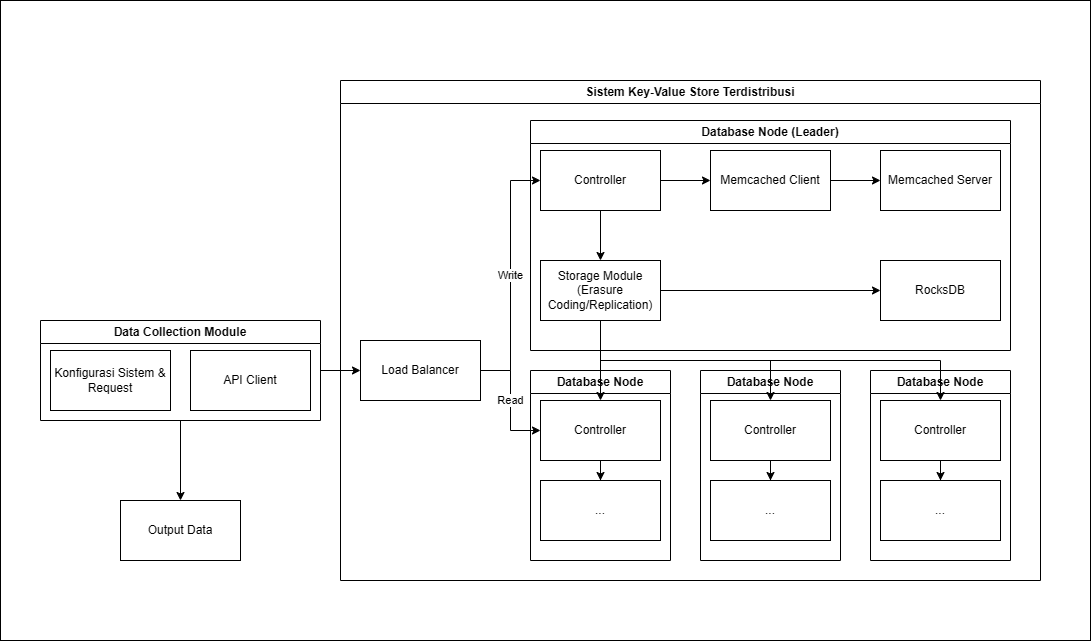
\includegraphics[width=0.95\textwidth]{resources/chapter-3/general-architecture.png}
    \caption{Struktur Komponen Komunikasi Antar-Node}
    \label{fig:node-communication-structure}
\end{figure}